\documentclass{article}
\usepackage{pgfplots}
\usepackage{filecontents}
\usepackage{verbatim}
\pgfplotsset{compat=1.8}
\usepackage{pgfplotstable}

\begin{document}

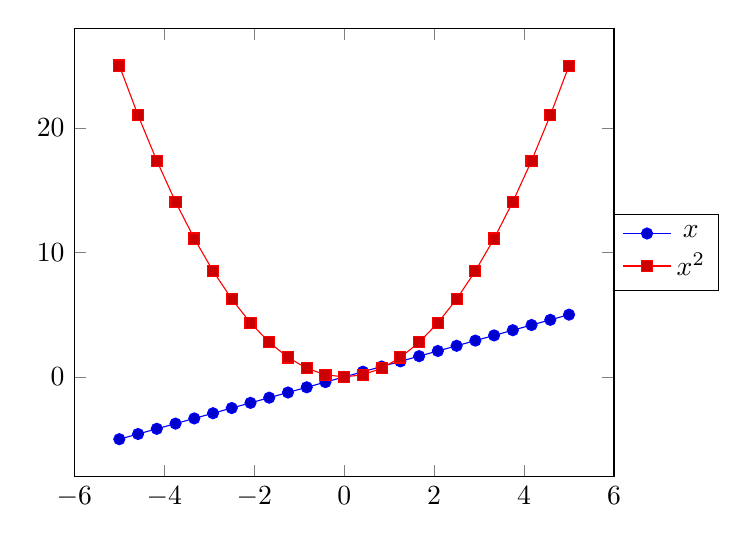
\begin{tikzpicture}
  \begin{axis}[
      legend entries={$x$,$x^2$},
      legend style={
        at={(1,0.5)},        % 1.03(>1) moves out of the graph along x, 0.5 means half-way along y
        anchor=west         %where the image will 'hang/support'. North/South/East/West means anchor will attach at ``at coordinate from top/bottom/right/left that direction. 
      }
    ]
    \addplot {x};
    \addplot {x^2};
  \end{axis}
\end{tikzpicture}
%%%%%%%%%%%%%%%%%%%%%%%%%%%%%%%%%%%%%%%%

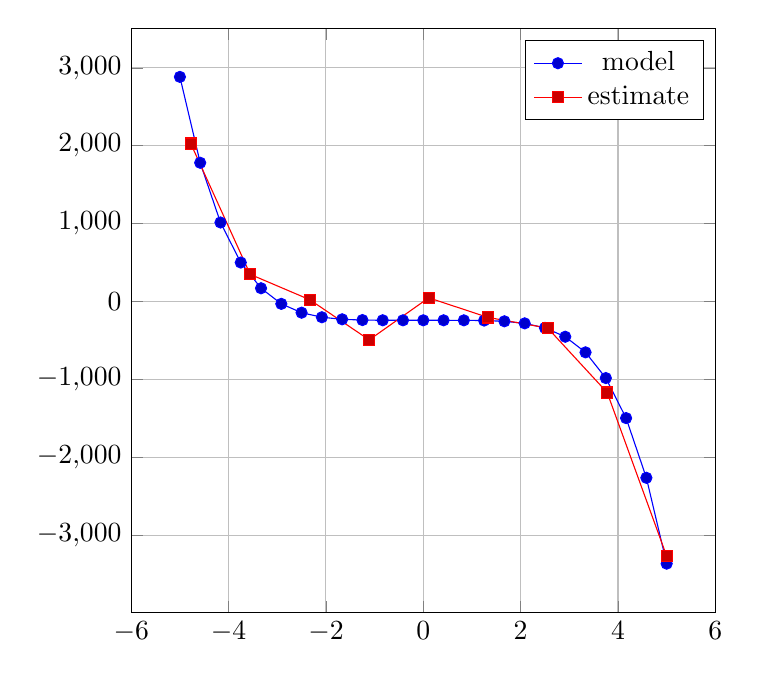
\begin{tikzpicture}
  \begin{axis}[
      height=9cm,
      width=9cm,
      grid=major,
    ]
    \addplot {-x^5 - 242};
    \addlegendentry{model}
    \addplot coordinates {
      (-4.77778,2027.60977)
      (-3.55556,347.84069)
      (-2.33333,22.58953)
      (-1.11111,-493.50066)
      (0.11111,46.66082)
      (1.33333,-205.56286)
      (2.55556,-341.40638)
      (3.77778,-1169.24780)
      (5.00000,-3269.56775)
    };
    \addlegendentry{estimate}
  \end{axis}
\end{tikzpicture}

%%%%%%%%%%%%%%%%%%%%%%%%%%%%%%%%%%%%%%%%
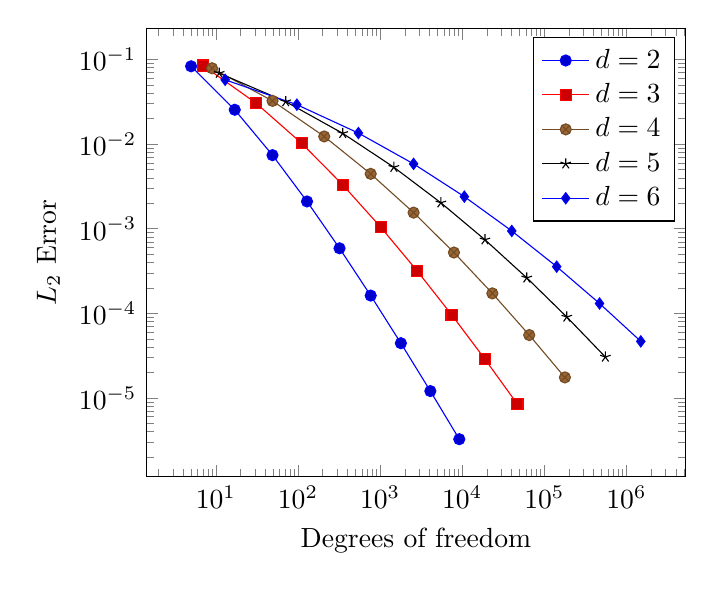
\begin{tikzpicture}
  \begin{loglogaxis}[
      xlabel={Degrees of freedom},
      ylabel={$L_2$ Error}
    ]
    \addplot coordinates {
      (5,8.312e-02)    (17,2.547e-02)   (49,7.407e-03)
      (129,2.102e-03)  (321,5.874e-04)  (769,1.623e-04)
      (1793,4.442e-05) (4097,1.207e-05) (9217,3.261e-06)
    };
    \addplot coordinates{
      (7,8.472e-02)    (31,3.044e-02)    (111,1.022e-02)
      (351,3.303e-03)  (1023,1.039e-03)  (2815,3.196e-04)
      (7423,9.658e-05) (18943,2.873e-05) (47103,8.437e-06)
    };
    \addplot coordinates{
      (9,7.881e-02)     (49,3.243e-02)    (209,1.232e-02)
      (769,4.454e-03)   (2561,1.551e-03)  (7937,5.236e-04)
      (23297,1.723e-04) (65537,5.545e-05) (178177,1.751e-05)
    };
    \addplot coordinates{
      (11,6.887e-02)    (71,3.177e-02)     (351,1.341e-02)
      (1471,5.334e-03)  (5503,2.027e-03)   (18943,7.415e-04)
      (61183,2.628e-04) (187903,9.063e-05) (553983,3.053e-05)
    };
    \addplot coordinates{
      (13,5.755e-02)     (97,2.925e-02)     (545,1.351e-02)
      (2561,5.842e-03)   (10625,2.397e-03)  (40193,9.414e-04)
      (141569,3.564e-04) (471041,1.308e-04) (1496065,4.670e-05)
    };
    \legend{$d=2$,$d=3$,$d=4$,$d=5$,$d=6$}
  \end{loglogaxis}
\end{tikzpicture}

\setlength{\fboxsep}{0pt}
\fbox{
  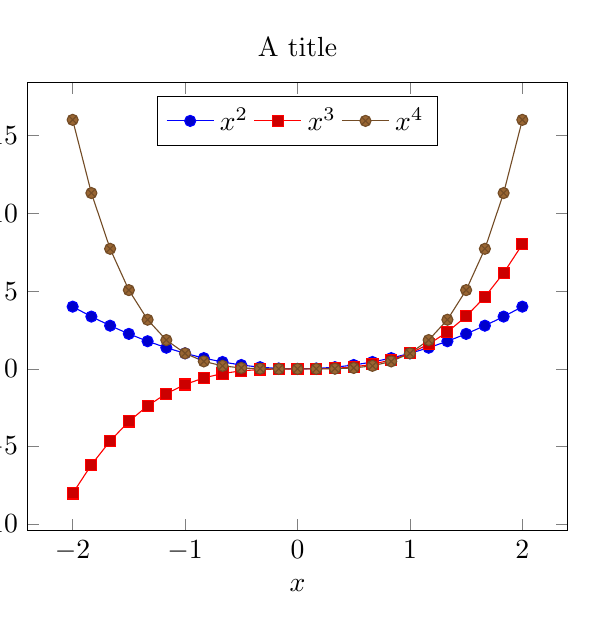
\begin{tikzpicture}
    \begin{pgfinterruptboundingbox}
      \begin{axis}[
          title=A title,
          xlabel={$x$},
          ylabel={$y$},
          legend style={at={(0.5,0.97)},
            anchor=north,legend columns=-1},
          domain=-2:2           % domain on the x axis
        ]
        \addplot {x^2};
        \addplot {x^3};
        \addplot {x^4};
        \legend{$x^2$,$x^3$,$x^4$}
      \end{axis}
    \end{pgfinterruptboundingbox}

    \useasboundingbox
    (current axis.below south west)
    rectangle (current axis.above north east);
  \end{tikzpicture}
}

\begin{tikzpicture}
  \begin{axis}[%
      scale only axis,
      width=0.45\textwidth,
      height=0.2\textheight,
      xmin=0, xmax=300,
      ymin=-2e+06, ymax=1e+07,
      legend entries={Analytic solution,GPS data,Kalman filtered},
      legend style={nodes=right},
      legend pos= south east]
    \addplot [color=blue, solid]
    coordinates{ (0,7e+06) (0.1,7.0007e+06) (0.2,7.0014e+06) };
    \addplot [color=green, solid]
    coordinates{ (0,6.99999e+06) (0.1,7.00071e+06) (0.2,7.00143e+06) };
    \addplot [color=red, solid]
    coordinates{ (0,0) (0.1,7.00071e+06) (0.2,7.00174e+06) };
  \end{axis}
\end{tikzpicture}


\begin{comment}
  :Title: Convergence Plot
  :Tags: PGFPlotstable;Mathematics;Manual
  :Author: Christian Feuersänger
  :Slug: convergence-plot

  We assume that we did some scientfic experiment.
  The scientific experiment yielded three
  input data tables: one table for each involved parameter
  d = 2, d = 3, d = 4. The data tables contain ``degrees
  of freedom'' and some accuracy measurement ``l2_err''. In addition,
  they might contain some meta-data
  (in our case a column ``level'').

  What we want is to produce three plots, each dof versus l2_err,
  in a loglog plot. We expect that
  the result is a line in a loglog plot, and we are interested in
  its slope log e(N) = -a log(N) because that
  characterizes our experiment.

  The code is from the PGFPlots 1.10 manual:
  ``3.3 Solving a Real Use Case: Scientific Data Analysis''.
\end{comment}

\begin{tikzpicture}
  \begin{loglogaxis}[
      title=Convergence Plot,
      xlabel={Degrees of freedom},
      ylabel={$L_2$ Error},
      grid=major,
      legend entries={$d=2$,$d=3$,$d=4$},
    ]
    \addplot table {../data/data_d2.dat};
    \addplot table {../data/data_d3.dat};
    \addplot table {../data/data_d4.dat};
    \addplot table[
      x=dof,
      y={create col/linear regression={y=l2_err,
          variance list={1000,800,600,500,400,200,100}}}
    ]
             {../data/data_d4.dat}
             % save two points on the regression line
             % for drawing the slope triangle
             coordinate [pos=0.25] (A)
             coordinate [pos=0.4]  (B)
             ;
             % save the slope parameter:
             \xdef\slope{\pgfplotstableregressiona}

             % draw the opposite and adjacent sides
             % of the triangle
             \draw (A) -| (B)
             node [pos=0.75,anchor=west]
             {\pgfmathprintnumber{\slope}};
  \end{loglogaxis}
  \begin{loglogaxis}[
      footnotesize,
      clip=false,
      xshift=7cm,
    ]
    \addplot table {../data/data_d2.dat}
    node [pos=1,pin=0:Special.] {}
    ;
  \end{loglogaxis}
\end{tikzpicture}

\end{document}
